\section{Information-Theoretic Metrics}

\subsection{Motivation for IT Metrics}

\begin{frame}
    \frametitle{Motivation for IT Metrics (1): The Rise of Multivariate Attacks}
    
     Side-channel analysis evolved beyond simple CPA to include powerful \textbf{multivariate attacks} like template attacks and linear regression analysis.
     \newline These advanced attacks can often recover a secret key with substantially fewer traces than their univariate counterparts.
   
    
    \begin{alertblock}{The Problem}
        Metrics like correlation and SNR are not easily extended to a multivariate setting. This created the need for new metrics that could fairly assess the risk posed by these stronger attacks.
    \end{alertblock}
\end{frame}

\begin{frame}
    \frametitle{Motivation for IT Metrics (2): Separating Device from Attacker}
    
  
    A key desire behind IT metrics was to distinguish between two separate concepts:
    \begin{enumerate}
        \item \textbf{The implementation:} a device and its countermeasures, which inherently leak information.
        \item \textbf{The attacker:} the specific methods and capabilities used to exploit that information.
    \end{enumerate}
  
    
        Instead of asking "Can my specific attack succeed?", IT metrics aim to answer:
        \vspace{0.3cm}
        
        \centering
        \textit{"How secure is this implementation against side-channel attacks in general?"}
        \vspace{0.3cm}
        
        This shifts focus away from attack-specific metrics (like SR and GE), allowing for more generic conclusions about the security of a device.
    
\end{frame}

\begin{frame}
    \frametitle{Information Theory Basics (1): Entropy}
    
    \begin{block}{Entropy H(X)}
        Entropy measures the average uncertainty of a random variable. Before an attack, we have an initial uncertainty about the secret key, $K$.
        
        For a discrete variable, it is defined as:
        $$ H(X) = - \sum_{x \in \mathcal{X}} \text{Pr}(X=x) \cdot \log_2(\text{Pr}(X=x)) $$
        The result is measured in \textbf{bits}.
    \end{block}
    
    \textbf{Example: An AES Key Byte} \newline
        If the secret key byte $K$ is uniformly random, there are 256 possibilities. The initial entropy is:
        $$ H(K) = \log_2(256) = 8 \text{ bits} $$
        This represents our total lack of knowledge before observing any leakage.
\end{frame}

\begin{frame}
    \frametitle{Information Theory Basics (2): Conditional Entropy}
    
    \begin{block}{Conditional Entropy $H(X|Y)$: Remaining Uncertainty}
        Conditional Entropy measures the uncertainty of a variable $X$ \textbf{given that you already know} the value of another variable $Y$.
        
        \vspace{0.3cm}
        
        \centering
        \textit{What is the remaining uncertainty of the key \textbf{K}, given that we have observed the leakage \textbf{L}?}
        
        \vspace{0.3cm}
        This is written as $\mathbf{H(K|L)}$. From a security perspective, we want this value to be as high as possible after an attack.
        $$H(X|Y)=-\sum_{x \in X, y \in Y}\text{Pr}(X=x,Y=y)\cdot\log(\text{Pr}(X=x|Y=y))$$
    \end{block}
\end{frame}

\begin{frame}
    \frametitle{Information Theory Basics (3): Continuous Variables}
    
  
        Since side-channel leakage is often an analog signal, we extend the concept of entropy to continuous random variables. 
        
        For a variable $X$ with a probability density function (PDF) Pr$(x)$, it is defined as:
        $$ H(X) = - \int_{X} \text{Pr}(X=x) \log_2( \text{Pr}(X=x)) \, dx $$
    
        The joint and conditional entropies for continuous variables `X` and `Y` are defined similarly:
        
        \textbf{Joint Entropy:}
        $$ H(X, Y) = - \iint_{X,Y} \text{Pr}(X=x, Y=y) \log_2 \text{Pr}(X=x, Y=y) \, dx dy $$
        
        \textbf{Conditional Entropy:}
        $$ H(X|Y) = - \iint_{X,Y} \text{Pr}(X=x, Y=y) \log_2 \text{Pr}(X=x|Y=y) \, dx dy $$
\end{frame}

\begin{frame}
    \frametitle{Information Theory Basics (4): Visual analogy}
    
    \begin{figure}
        \centering
        \includegraphics[width=0.8\textwidth]{placeholder.png} 
        \caption{Visualization of information-theoretic concepts with Venn diagrams.}
    \end{figure}
    
    %\begin{itemize}
    %    \item \textbf{H(K)} and \textbf{H(L)} represent the total uncertainty (entropy) of the key and the leakage, respectively.
    %    \item The \textbf{overlap} represents the \textbf{Mutual Information, I(K;L)}—the information they share.
    %    \item The part of H(K) that \textit{does not} overlap is the \textbf{Conditional Entropy, H(K|L)}—the uncertainty about the key that remains even after seeing the leakage.
    %\end{itemize}
\end{frame}

\subsection{Mutual Information}
\begin{frame}
    \frametitle{Mutual Information}
    
    \begin{block}{Definition}
        Mutual Information quantifies the amount of information that one variable ($Y$) provides about another ($X$). It is the \textbf{reduction in uncertainty} of $X$ after observing $Y$.
        
        It is fundamentally defined by the relationship between the entropies:
        $$ I(X;Y) = H(X) - H(X|Y) $$Theory
    \end{block}
    
    When applied to our problem, the formula becomes:
    $$ I(K;L) = H(K) - H(K|L) $$
    $$ \text{Information Leaked} = \text{Initial Uncertainty} - \text{Remaining Uncertainty} $$
    This metric, $I(K;L)$, represents the total amount of information (in bits) that the leakage $L$ reveals about the secret key $K$.
 
\end{frame}

\begin{frame}
    \frametitle{Mutual Information: Expanded Formulas}

    For discrete random variables $X$ and $Y$:
    $$
    I(X; Y) = \sum_{x \in X} \sum_{y \in Y} \Pr(X = x, Y = y) \cdot \log_2 \left( \frac{ \Pr(X = x, Y = y) }{ \Pr(X = x)\Pr(Y = y) } \right)
    $$


    For continuous random variables $X$ and $Y$ (using probability density functions):
    $$
    I(X; Y) = \int_{X} \int_{Y} \Pr(X = x, Y = y) \cdot \log_2 \left( \frac{ \Pr(X = x, Y = y) }{ \Pr(X = x)\Pr(Y = y) } \right) dx\,dy
    $$

    Mixed Case (Discrete $X$, Continuous $Y$)
        $$
        I(X; Y) = \sum_{x \in X} \int_{Y} \Pr(X = x, Y = y) \cdot \log_2 \left( \frac{ \Pr(X = x, Y = y) }{ \Pr(X = x)\Pr(Y = y) } \right) dy
        $$
\end{frame}


\begin{frame}
    \frametitle{Mutual Information: Visual Analogy}
    
    \begin{figure}
        \centering
        \includegraphics[width=0.8\textwidth]{placeholder.png} 
        \caption{Visualization of MI with Venn diagrams.}
    \end{figure}
    
    %\begin{itemize}
    %    \item \textbf{H(K)} and \textbf{H(L)} represent the total uncertainty (entropy) of the key and the leakage, respectively.
    %    \item The \textbf{overlap} represents the \textbf{Mutual Information, I(K;L)}—the information they share.
    %    \item The part of H(K) that \textit{does not} overlap is the \textbf{Conditional Entropy, H(K|L)}—the uncertainty about the key that remains even after seeing the leakage.
    %\end{itemize}
\end{frame}


\begin{frame}
    \frametitle{Applying MI to Side-Channels}
    
        We want a metric that can capture \textbf{multivariate leakages}. To do this, we move from thinking about a single leakage value $L$ to a leakage \textbf{vector} $\mathbf{L}$.
        
        \vspace{0.3cm}
        
        The goal is to use Mutual Information to quantify how many bits of information we can learn about the secret key $K$ by observing the multivariate side-channel leakage vector $\mathbf{L}$.
    
    \begin{alertblock}{}
        The definition remains the same, but the variables now have a specific meaning:
        $$ I(K;\textbf{L}) = H(K) - H(K|\textbf{L}) $$
        $$ \text{Information Leaked} = \text{Initial Uncertainty} - \text{Uncertainty after the Attack} $$
    \end{alertblock}
\end{frame}

\begin{frame}
    \frametitle{The MI Formula for Side-Channels}
    
        Applying the definitions of entropy and Bayes' rule, the MI between the key $K$ and the leakage $\mathbf{L}$ can be expressed as:
        
        $$ I(K;\mathbf{L}) = - \sum_{k \in K} \Pr(k)\log_2\Pr(k) + \sum_{k \in K} \Pr(k) \int_{\mathbf{l} \in \mathbb{R}^m} \Pr(\mathbf{l}|k) \log_2 \Pr(k|\mathbf{l}) \, d\mathbf{l} $$
    
    \begin{block}{What we need to compute}
        To solve this, an evaluator needs to know several quantities:
        \begin{itemize}
            \item The key probability, $\Pr(k)$.
            \item The conditional leakage probability, $\Pr(\mathbf{l}|k)$.
            \item The posterior key probability, $\Pr(k|\mathbf{l}) \rightarrow$ we can get rid of this thanks to Bayes
        \end{itemize}
    \end{block}
\end{frame}

\begin{frame}
    \frametitle{Simplifying the MI Formula}
    
        In the very common case where the secret key $K$ is \textbf{uniformly random}:
        \begin{itemize}
            \item The probability of any specific key is $\Pr(k) = 1 / |K|$.
            \item The initial entropy is simply $H(K) = \log_2 |K|$.
        \end{itemize}
    
    \begin{block}{Simplified Formula}
        Under this assumption, the MI formula simplifies significantly:
        $$ I(K;L) = \log_2|K| + \frac{1}{|K|} \sum_{k \in K} \int_{\mathbf{l} \in \mathbb{R}^m} \Pr(\mathbf{l}|k) \log_2  \frac{\Pr(\mathbf{l}|k)}{\sum_{k^* \in K} \Pr(\mathbf{l}|k^*)}  dl $$
    \end{block}
\end{frame}

\begin{frame}
    \frametitle{}
    
    \begin{alertblock}{}
        After all the simplification, the formula reveals that the \textbf{only remaining quantity} the evaluator needs to compute is:
        
  
        $$\Pr(\mathbf{l}|k)$$
        
   
        This term is the likelihood of observing a side-channel leakage vector $\mathbf{l}$, given a certain key $k$.
    \end{alertblock}
    
    \begin{block}{}
        The computation of this quantity is directly linked to \textbf{leakage profiling}, \textbf{leakage modeling} and parameter estimation.
    \end{block}
\end{frame}

\begin{frame}
    \frametitle{Modeling the Leakage to Compute $\Pr(\mathbf{l}|k)$}
    
        To find a value for $\Pr(\mathbf{l}|k)$, we create a statistical model of the leakage. A common approach, known as a \textbf{univariate template}, assumes the leakage for each key $k$ follows a \textbf{Normal (Gaussian) Distribution}.
        
        \begin{enumerate}
            \item This model is built using the workflow of a profiled attack, so the evaluator can use an open device to measure traces $[L_0^{prof},L_1^{prof},\dots,L_{255}^{prof}]$
            \item For normal distributions, leakage modeling is equivalent to estimating the mean ($\mu_k$) and standard deviation ($\sigma_k$) from the set of profiling traces.
            \item This gives us a list of leakage models $[\mathcal{N}(\mu_0, \sigma_0), \dots, \mathcal{N}(\mu_{255}, \sigma_{255})]$.
        \end{enumerate}
\end{frame}

\begin{frame}
    \frametitle{The Univariate Template}
    
    \begin{block}{}
        With the univariate template assumption, the probability of observing leakage $\mathbf{l}$ for a given key $k$ is given by the Gaussian probability density function:
        
        $$ \Pr(l|k) = \frac{1}{\sigma_k\sqrt{2\pi}} e^{ -\frac{1}{2} \left( \frac{l-\mu_k}{\sigma_k} \right)^2 } $$
    \end{block}
    
    By plugging this concrete model for $\Pr(l|k)$ into the simplified MI formula we saw earlier, we can now calculate a numerical value for the information leakage.
    $$I(K;L) = \log_2|K| + \frac{1}{|K|} \sum_{k \in K} \int_{-\infty}^{+\infty} \Pr(l|k) \log_2  \frac{\Pr(l|k)}{\sum_{k^* \in K} \Pr(l|k^*)}  dl $$
\end{frame}


%%% MAYBE aggiungere dettagli sull'implementazione Sbox masked
\begin{frame}
    \frametitle{Using MI to make projections on security}

    Mutual Information allows deriving security bounds, projecting the number of traces an attacker would need for key recovery.
    
    \textbf{Unprotected Implementation:}
    $$ \text{Number of traces} \ge \frac{H(K)}{I(L;K)} $$
    
    \textbf{d-th Order Masked Implementation:}
    $$ \text{Number of traces} \ge \frac{H(Y_i)}{I(L_i;Y_i) \cdot d} $$

    \begin{alertblock}{}
        These formulas are approximations that may overestimate an attacker's capabilities. However, because MI is inherently multivariate, they can provide a more fair security picture than correlation-based shortcuts.
    \end{alertblock}
\end{frame}

\begin{frame}
    \frametitle{Visualizing Security with MI}
    
    The value of MI directly reflects the security of a device, independent of any specific attacker's scores or ranks.
    
    \begin{itemize}
        \item \textbf{High MI} $\implies$ High information leakage $\implies$ Low security.
        \item \textbf{Low MI} $\implies$ Low information leakage $\implies$ High security.
    \end{itemize}

    \begin{figure}
        \centering
        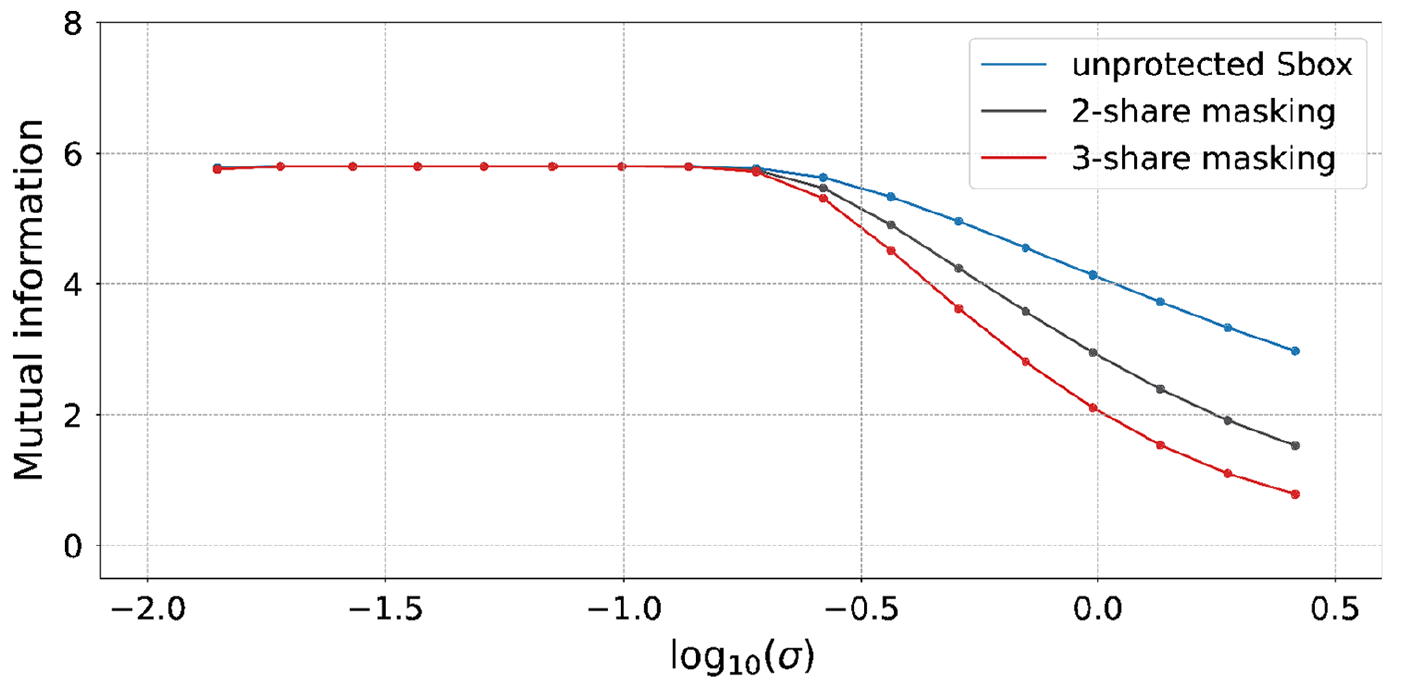
\includegraphics[width=0.8\textwidth]{metrics/Pictures/MI_masking.png}
        \caption{MI decreases as noise increases. Masking further amplifies this effect, showing its effectiveness as a countermeasure.}
    \end{figure}
\end{frame}




\subsection{Hypothetical Information}

\begin{frame}
    \frametitle{The Leakage Model: Two Scenarios}
    
    \begin{block}{Scenario 1: Theoretical Analysis (True Parameters)}
        Sometimes, an evaluator wants to test a countermeasure against a \textbf{theorized leakage model} without using experimental traces.
        \begin{itemize}
            \item \textbf{Example:} Assessing the security of a masking scheme against a perfect, non-linear leakage model.
            \item In this case, the model parameters (e.g., $\mu, \sigma$) are not estimated, but are \textbf{chosen} by the evaluator. These are considered the \textit{true parameters} for the theoretical model.
        \end{itemize}
    \end{block}
    
    \begin{block}{Scenario 2: Practical Evaluation (Estimated Parameters)}
        This is the case we discussed before. An evaluator uses a set of experimental profiling traces, $L_k^{prof}$, to \textbf{estimate} the model parameters ($\hat{\mu}, \hat{\sigma}$).
    \end{block}
\end{frame}

\begin{frame}
    \frametitle{Introducing Hypothetical Information (HI)}
    
    \begin{block}{Distinction in Terminology}
        To separate these two scenarios, the following terms are used:
        \begin{itemize}
            \item \textbf{Mutual Information (MI):} The metric calculated using \textbf{true parameters} from a theoretical leakage model. This achieves the goal of separating the implementation from the adversary.
            
            \item \textbf{Hypothetical Information (HI):} The metric calculated using \textbf{estimated parameters} ($\hat{\mu}, \hat{\sigma}$) from a real profiling dataset. This is what's computed in a practical evaluation.
        \end{itemize}
    \end{block}
    
    
\end{frame}

\begin{frame}
    \frametitle{The Pitfalls of Hypothetical Information (HI)}
    
        Unfortunately, an attacker's poor modeling is not fully reflected in the HI metric, which leads to two major types of errors.
    
    \begin{columns}[T] % Splits the frame into columns
        \begin{column}{0.5\textwidth}
            \textbf{1. Estimation Errors}
            \begin{itemize}
                \item Occur when the model is correct, but trained on \textbf{too few traces}.
                \item The resulting model is weak and may fail in a real attack.
                \item HI will still be positive and suggest that key recovery is possible, even when it is not.
            \end{itemize}
        \end{column}
        
        \begin{column}{0.5\textwidth}
            \textbf{2. Assumption Errors}
            \begin{itemize}
                \item Occur when the \textbf{chosen model is wrong} and does not reflect the device's actual leakage behavior.
                \item This can happen due to non-linear effects, measurement drift, or device differences.
                \item Even with infinite training data, the model is flawed. Yet, HI will likely be positive, suggesting an attack is possible when it's not.
            \end{itemize}
        \end{column}
    \end{columns}
\end{frame} 

\subsection{Perceived Information}

\begin{frame}
    \frametitle{The Fundamental Flaw of HI}
    
    The problem with HI is that it never \textbf{tests its own model against reality}.
        \begin{itemize}
            \item HI is calculated using only the profiling and modeling steps.
            \item It never considers a \textbf{test dataset} to see if the model's predictions actually match the device's real leakage.
            \item HI is "the amount of information that would be leaked from an implementation of which the leakages would be \textit{exactly predicted}" by the model.
        \end{itemize}
    
    
    \begin{alertblock}{}
    HI does not test its estimated model against the actual device leakage. \newline
        This gap is filled by a new metric that explicitly compares the model to reality: \textbf{Perceived Information (PI)}.
    \end{alertblock}
\end{frame}

\begin{frame}
    \frametitle{Cross Entropy}
    
    \begin{block}{}
        PI is built on the idea of \textbf{cross-entropy} $H_{p,q}(K|\mathbf{L})$. It measures the performance of a model distribution $q$ when it's used to describe a true distribution $p$.
        
        \begin{itemize}
            \item The \textbf{model distribution $q$} is our estimated model, $\hat{Pr}_{model}(\mathbf{l}|k)$, built from the profiling traces.
            \item The \textbf{true distribution $p$} is the actual leakage of the device, which we can only sample using a \textbf{ test data set}.
        \end{itemize}
    \end{block}
\end{frame}

\begin{frame}
    \frametitle{Introducing Perceived Information (PI)}
     \begin{block}{PI Definition}
        Perceived Information is defined as:
        $$ PI(\mathbf{L};K) = H(K) - H_{true, model}(K|\mathbf{L}) $$
        It subtracts the \textit{cross-entropy} between the true leakage and the model from the initial key entropy.
    \end{block}
    $$ PI(\mathbf{L};K) = (-\sum_{k \in K}\Pr(k)\log_2\Pr(k))-(-\sum_{k \in K,l \in L}\Pr_{true}(k|\mathbf{l})\log_2\hat{\Pr}_{model}(k|\mathbf{l})) $$
\end{frame}

\begin{frame}
    \frametitle{Computing PI}
   
        Assuming uniformly random keys and applying Bayes' rule, we get the general formula for Perceived Information:
        $$ PI(L;K) = H(K) + \sum_k \Pr(k) \sum_{l \in L_{k}^{test}} \Pr_{true}(l|k) \log_2 \left( \frac{\hat{\Pr}_{model}(l|k)}{\sum_{k^*} \hat{\Pr}_{model}(l|k^*)} \right) $$
    
    \begin{block}{}
        \begin{itemize}
            \item Computing $\hat{\Pr}_{model}(l|k)$ is identical to the computation of $\hat{\Pr(l|k)}$ in the HI metric
            
            \item To compute $\Pr_{true}(k|l)$  we distinguish between \textbf{simulated leakage} and \textbf{real traces}
        \end{itemize}
    \end{block}
\end{frame}

\begin{frame}
    \frametitle{Case 1: PI with Simulated Leakage}
    
    \begin{block}{Theoretical Scenario}
        In a theoretical analysis, the evaluator can \textbf{define} the true leakage distribution. For example, simulated traces can be generated with known characteristics (known noise level, ...).
        
        \begin{itemize}
            \item Here, $\Pr_{true}(l|k)$ is known because the evaluator created it.
            \item The PI metric then quantifies how well the estimated model, $\hat{\Pr}_{model}$, can capture this known, true distribution.
        \end{itemize}
    \end{block}
    
    \begin{alertblock}{}
        This scenario answers the question: \textit{"Is my training process good enough to learn this specific kind of leakage?"}
        
        A negative PI value in this case clearly indicates an \textbf{estimation error} (e.g., not enough training traces).
    \end{alertblock}
\end{frame}


\begin{frame}
    \frametitle{Visualizing Security with PI}
   \begin{figure}
        \centering
        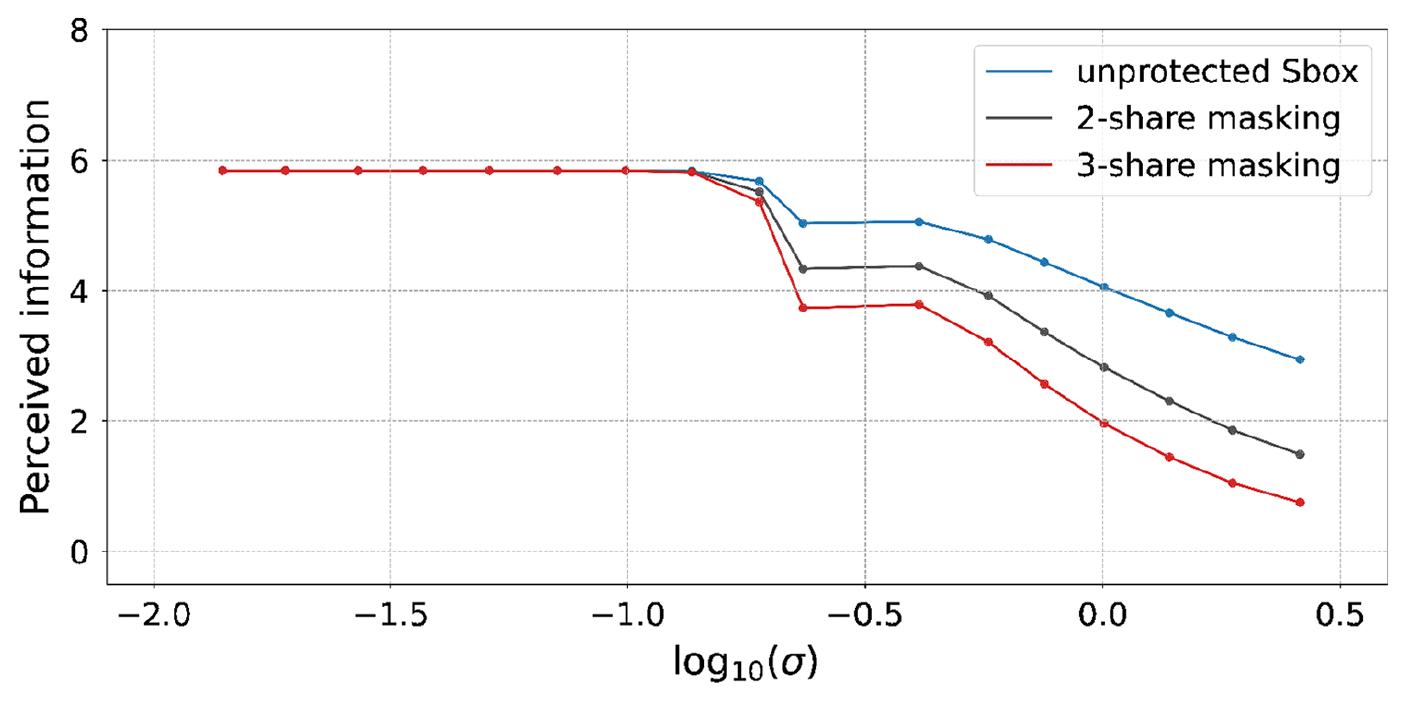
\includegraphics[width=0.8\textwidth]{metrics/Pictures/PI_masking.png}
        \caption{PI is positive and decreases as artificial white noise increases. The model training adequately captures the simulated leakage}
    \end{figure}
\end{frame}


\begin{frame}
    \frametitle{Case 2: PI with Real Traces}
    
    \begin{block}{Practical Scenario}
        In a practical evaluation of a real device, the true distribution is unknown. We can only \textbf{sample} it by collecting a \textbf{test dataset}, $L_k^{test}$.
        
        \begin{itemize}
            \item For each possible key $k$, we capture a new set of $n_k$ test traces.
            \item Sampling from the test set implies that the probability of observing any specific trace $l$ from that set is $\Pr_{true}(l|k) = 1/n_k$.
        \end{itemize}
    \end{block}
    
    \begin{alertblock}{The Practical PI Formula}
        This leads to the final, practical formula for PI:
        $$ PI(L;K) = H(K) + \sum_{k \in K} \frac{\Pr(k)}{n_k} \sum_{l \in L_k^{test}} \log_2 \left( \frac{\hat{\Pr}_{model}(l|k)}{\sum_{k^* \in K} \hat{\Pr}_{model}(l|k^*)} \right) $$
    \end{alertblock}
\end{frame}

\begin{frame}
    \frametitle{Comparison: Real and Simulated traces}
    
    \begin{block}{What Practical PI tells us}
        This metric directly answers the most important question for an evaluator:
        \vspace{0.3cm}
        
        \centering
        \textit{"Does my trained model capture the \textbf{actual device leakage} well enough to be useful?"}
    \end{block}
    
    \begin{block}{Detecting Errors}
        \begin{itemize}
            \item Unlike MI and HI, \textbf{PI can be negative}.
            \item A negative PI value proves that key recovery is not possible with the current model. It serves as a clear indicator of:
                \begin{itemize}
                    \item \textbf{Estimation errors} (not enough training data)
                    \item OR \textbf{Assumption errors} (the model is fundamentally wrong)
                \end{itemize}
        \end{itemize}
    \end{block}
\end{frame}

\begin{frame}
    \frametitle{Summary: The Hierarchy of IT Metrics}
    
        The three information-theoretic metrics are bound by the following important inequality:
        
        \vspace{1cm}
        \begin{itemize}
            
        \centering
        \huge
        $ PI \le MI \le HI $
        
        \end{itemize}{}
        \vspace{1cm}
    
    \begin{alertblock}{}
        The security bounds we saw earlier (for estimating the number of traces) can be computed with any of these metrics, but a calculation using PI is only meaningful \textbf{if the PI value is positive}.
    \end{alertblock}
\end{frame}

\subsection{Limitations of IT Metrics}

\begin{frame}
    \frametitle{Limitations of Information-Theoretic Metrics}
    
    \begin{enumerate}
        \item \textbf{Requires Generative Models:}
        The need for a probabilistic generative model (one that can describe the full leakage distribution) can exclude powerful discriminative models, like many neural network classifiers.
        
        \vspace{0.3cm}
        
        \item \textbf{Computational Hardness with High Dimensions:}
        IT metrics are naturally multivariate, but computing the required multi-dimensional integrals becomes extremely difficult as the number of leakage samples $m$ or masking shares $d$ increases.
        
        \vspace{0.3cm}
        
        \item \textbf{Difficulty with Horizontal Attacks:}
        Combining the leakage from multiple different intermediate values in the cipher (e.g., Sbox input and output) also dramatically increases the dimensionality and computational complexity.
    \end{enumerate}
    
    
        To resolve these issues evaluators often turn to techniques like Monte-Carlo integration, dimensionality reduction, or other approximations.
\end{frame}
